
\section{Desarrollo del Trabajo} 

\begin{enumerate}[1.]
         

	\item Resumen

  Para el presente trabajo se tomo referencia el como esta estructurada la base de datos de la bibilioteca universitaria, se diseño la base datos con las clases requeridas para el trabajo y posteriormente se analiz\'o base de datos para encontrar la tabla de hechos en este caso se considero como tabla de hechos a la tabla RESERVA, como segundo se identific\'o la granulidad y las tablas dimensionales, luego se realizar\'on las consultas respectivas para hallar los indicadores requeridos.
\\
	\item Objetivo

 El objetivo principal de este trabajo es apoyar a las consultas de los usuarios finales en un almacén de datos. Se orienta entorno a la comprensibilidad y rendimiento para obtener informcaci\'on objetiva para tomar las desiciones con el menor porcentaje de errores.
\\	
	\item Listado de Indicadores
	
-  Porcentaje de profesores y estudiantes del progrma de utiliza los recursos bibliograficos disponibles en la escuela de sistemas, por curso y ciclo

-  porcentaje de referencias  bibliograficas de los trabajos de investigacion de la escuela de sistemas que utiliza los recursos bibliograficos disponibles

- Porcentaje de referencias  bibliograficas  de los silabos de los cursos de la escuela  de sistemas que utiliza recurdsos bibliograficos.
\\	
	
	\item Diseño de Modelo multidimensional
	
- Modelo proyectado de la Base de Datos:
	\begin{center}
	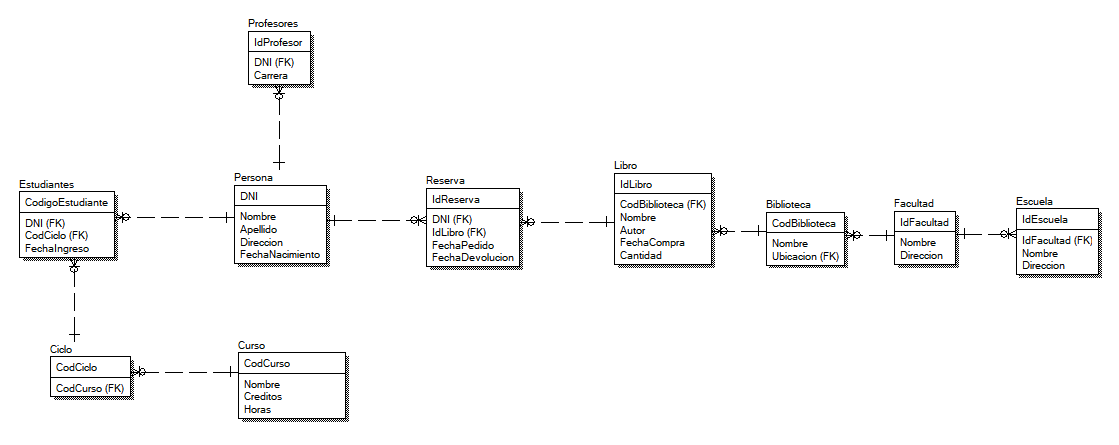
\includegraphics[width=17cm]{./Imagenes/BD_biblioteca} 
	\end{center}

- ModeloDimensional de la Base de Datos:
	\begin{center}
	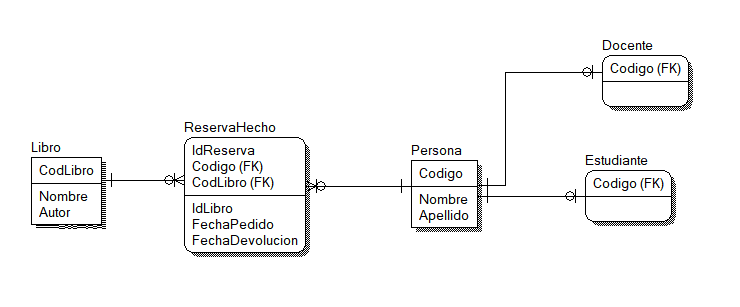
\includegraphics[width=17cm]{./Imagenes/bdDimensional} 
	\end{center}

- Consultas propuestas:
\\
1. Query:

2. Query:

3. Query:


	\item Bibliograf\'ia
\\
- https://es.wikipedia.org/wiki/Modelado\_dimensional
\\
- https://blog.bi-geek.com/modelo-dimensional/
\\
- https://searchdatacenter.techtarget.com/es/definicion/Base-de-datos-multidimensional-MDB
\\
- https://es.calameo.com/books/002299301667571c7ab05
\\
-https://searchdatacenter.techtarget.com/es/consejo/Tablas-de-dimension-vs-tablas-de-hechos-Cual-es-la-diferencia


\end{enumerate} 
